\documentclass{acm_proc_article-sp}

\usepackage{url}
\usepackage{epstopdf}
\usepackage{datetime}

% Switch between these two to add/remove todo comments
\usepackage{color}
\newcommand{\todo}[2]{{\color{red}\textbf{#2}}}
%\newcommand{\todo}[2]{#1}

\usdate
\settimeformat{ampmtime}

\begin{document}

\title{Improving Usability of Remote Access to Sensitive Data}

\author{
Draft Copy: \today\ \currenttime
}

%\numberofauthors{2} 
%
%\author{
%\alignauthor Alexander Crowell \\
%       \affaddr{Computer Science and Engineering Division}\\
%       \affaddr{University of Mighigan}\\
%       \affaddr{Ann Arbor, MI, USA}\\
%       \email{crowella@umich.edu}
%\alignauthor Atul Prakash \\
%       \affaddr{Computer Science and Engineering Division}\\
%       \affaddr{University of Mighigan}\\
%       \affaddr{Ann Arbor, MI, USA}\\
%       \email{aprakash@umich.edu}
%}

\maketitle
\begin{abstract}

As we enter an era of ``big data", where analysis of large-scale data is
revealing important insights into a variety of fields, there is an ever greater
demand for access to new data wherein the potential for new insights may lie.
However, in many cases, this need for access conflicts with the desire to
protect data privacy.  Indeed, many types of important data present just such a
dilemma, including copyrighted data, personal information of individuals, and
data containing state or corporate secrets.

In this paper, we propose Data Capsules, a system that is designed to enable
access to sensitive data for analysis by trusted remote users, while
maintaining reasonable guarantees of data security.  Data Capsules uses
virtualization to provide remote users with a privileged, but secure
environment into which they can bring arbitrary, and even potentially
malicious, software or data in order to analyze sensitive data, while
minimizing the available channels for data leaks.  Our early implementation
realizes much of this protection, providing a basic framework for secure
analysis of data that addresses many aspects of network, storage, and covert
channel security.

\end{abstract}

\category{D.4.6}{Operating Systems}{Security and Protection}
\category{H.3.4}{Systems and Software}{Distributed Systems}[cloud computing, data capsules]

\keywords{data capsules, data privacy}

\section{Introduction}

In the age of the Internet, new data is being created at incredible rates
\cite{digital-universe}.  Along with these waves of new data, new tools have
in turn been created to help analyze and gain insight from it. Unfortunately,
access to data is not always a simple matter.  Some types of data may be
sensitive, including data protected by copyright, data representing the personal
information of individuals, as well as any data that may contain secrets that
its owner does not wish to have revealed, for example corporate or state secrets.

The current state-of-the-art \cite{vrdc} in systems developed for the purpose
of enabling access to these types of data use remotely accessed machines, which
can then be used by researchers without the need for travel to conduct their
analysis. But beyond this apparent convenience, rules for using such systems
are often highly restrictive, with researchers limited to using predefined
software environments, and being subject to strict auditing requirements for
all software and data that is uploaded to these software environments.  

To solve this substantial inconvenience, we propose a new system which we call
Data Capsules.  While, to an end user, a Data Capsules environment will
minimally differ from the type of environment provided by the CMS Virtual
Research Data Center, its design grants end users privileged access to install
software of their choice --- even down to the virtualization-compatible
operating system of their choice --- without requiring a review process and
without any compromise to the security of the data being provided.

Data Capsules makes use of virtualization as a key element in achieving this
security and usability goal.  Under the Data Capsules use model, a researcher
would be allocated a virtual machine (henceforth abbreviated as VM, or guest
VM), which they could then prepare and maintain with whatever software and
underlying operating system is best suited to the intended purpose.  Each Data
Capsules VM is endowed with two modes of operation.  In \emph{maintenance} mode,
the researcher is endowed with full Internet access, which enables them to
easily configure and maintain the software environment almost as if they were
using a their own personal machine; however, in maintenance mode, the researcher
does not have access to the sensitive data.  In order to gain access to this
data, the user must switch their VM to the second mode, which we call
\emph{secure} mode.  In secure mode, the user's VM state is saved, and
execution continues on an alternate machine that is firewalled to prevent
Internet access, but which does have access to the sensitive data.

In this manner, once a user has configured their system and is prepared to
run their analysis on the data, they simply switch to secure mode and start
the analysis.  Any results obtained from this analysis can then be stored in a
designated \emph{secure storage volume}, which is only attached to the VM in
secure mode.  Since this result data is only accessible in secure mode, it
follows that data can only be released from the virtual environment when in
secure mode.

When a user wishes to further change their software environment in order to
continue data analysis, they may then switch back to maintenance mode, after
which the secure storage volume will detatch, and all VM state since the
previous switch to secure mode is discarded, with the VM continuing to run from
the point it left off at when last in maintenance mode.  In this way, every
trace of the operations performed on the sensitive data is erased and forgotten.

Furthermore, assuming any sensitive data is read-only, and is properly backed
up, Data Capsules functionality means that there is no need to audit installed
software for malware, as even infected software would be unable to exfiltrate
the data from the secure mode environment.

In the following sections, we discuss related work, elaborate on the design and
implementation of the Data Capsules system, and discuss the current state of
the project and potential directions for future work.

\section{Related Work}

As mentioned, in addition to research systems for securing data, there are
several real-world systems that address the issue of securing sensitive data.
In this section, we discuss a selection of both real-world implementations of
such systems as well as systems proposed by the academic community.

\subsection{Real-World Systems}

Systems that enable supervised and audited computational research of sensitive
data date back at least as far as the 1990s, when a Census Research Data Center
was opened in Boston.  Since the opening of this initial office, the U.S.
federal government has established several Research Data Centers (RDCs)
\cite{census-rdc} across the country to enable researchers access to
unpublished Census data for the purpose of conducting research that could
provide beneficial guidance to public policy.

Potential researchers must first submit a research proposal demonstrating
scientific merit and potential benefit to Census Bureau programs.  Once granted
access, a researcher then visits one of the CRDCs in person, and, after swearing
to protect data confidentiality, will then be permitted to use preallocated
machines inside the facility with a preloaded suite of software in order to
conduct their research.  Upon completion of their research, their results are
human-audited to protect confidentiality, and then released.

While this system provides access to Census data, and seems robust to data
leaks, it is also highly restrictive, requiring researchers to relocate and use
foreign hardware and potentially software as well, to conduct their research.

More recently, the Centers for Medicare and Medicaid Services began providing
Medicare and Medicaid data using the CMS Virtual Research Data Center (VRDC) in
2013 \cite{vrdc}.  VRDC provides a more flexible model by allowing researchers
to remotely access desktop environments provided by a cloud infrastructure.
This model relieves researchers of the need to travel to a physical location,
and also avoids the security risk of researchers having to receive and
safeguard physical copies of the data while they are conducting their research,
as was formerly the case.

However, this state-of-the-art solution still suffers from significant
drawbacks, in that researchers are largely limited to using the preallocated
environments supplied by the VRDCs.  In order to upload software or data not
already available in a virtual desktop, it must first undergo a manual review
process.  For large software suites, this can at best add significant
inconvenience, and at worst expose the system to a malicious attack, as there is
no method for reliably detecting malicious software.  Data Capsules is designed
so that no review process is necessary to upload software or data to an
environment, while providing strong guarantees of data privacy by design.

\subsection{Systems Using Virtualization}

QubesOS \cite{qubes} is a system for isolating a user's desktop environment into
secure compartments, called ``Qubes," which are intended to prevent malicious
code from compromising the entire system by restricting its effect to the
compartment in which it resides.  Although Qubes is very effective for this 
purpose, it would not serve as a particularly secure tool for data access, as it
suffers from the same challenge of how to move data from one compartment, which
is presumably unrestricted, into another compartment containing the sensitive
data to be operated on.  Data Capsules offers a clear design for allowing the
import of data and code into an environment that can still offer secure access
to sensitive data.

Storage Capsules \cite{capsules-borders} is a virtualization-based system for
protecting data privacy on individual machines.  Under Storage Capsules, a
machine runs a virtual machine manager (VMM) system, which in turn runs the
user's operating system environment within a VM.  On the same machine, there is
a second VM running an interface that serves as a ``storage capsule" for
sensitive data.  The user's main VM is endowed with two modes of operation,
\emph{normal} and \emph{secure} mode, and similar to Data Capsules, normal mode
grants full network priviliges while secure mode grants access to the sensitive
data, via communication with the storage capsule VM.

While our work shares the dual-mode user interface of Storage Capsules, the
differences largely end there.  Our system is designed under a significantly
different usage model, in which end users are accessing the VM remotely and
operating on data stored outside of the machine a VM resides on. This different
environment substantially alters the threat model, and provides a different set
of channels for potential data leaks.  As a result, Data Capsules offers the
potential to provide an environment for data access that is faster and more
robust to data leaks.

\subsection{Information Flow Control}

Mandatory access control systems, such as SELinux \cite{selinux}, offer the
ability to place strict controls on how a system is used.  It is conceivable
that a machine could be configured with a policy that would enable users to
analyze sensitive data without a high risk of data leakage.  However, such a
policy would have to be written and maintained by an expert, in order to account
for each piece of software that is to operate on the data, and the policy would
likely be so large and complex that it would be hard to avoid at least some
security errors.  Because of this, it is not a particularly flexible solution,
and would still require manual action before a user could begin using their own
custom software in such an environment.

Specialized operating systems that enforce information flow control, such as
HiStar \cite{histar}, offer low-level operating system primitives that allow
developers to design programs in such a way that data leaks are not possible.
As with SELinux, there is still a substantial burden of having to craft policies
that prevent these malicious data flows.  Additionally, programs must be
specifically developed for compatibility with HiStar, creating an even greater
burden on users so long as that system is not widely supported by the software
community.

\section{Design}

We now discuss the design of the Data Capsules system.  This includes the
functional requirements for the two modes of operation and a discussion of how
the system avoids various channels for leaking data.

\subsection{Security Goals and Threat Model}
\label{sec:Threat Model}

The goal of the Data Capsules system is to provide a usable environment for data
analysis that also provides a reasonably strong (as we elaborate on below)
guarantee of data privacy from parties other than the end user to whom a VM
belongs.  Data Capsules is not designed to provide any protection to the
integrity of sensitive data.  This is assumed trivial, as the sensitive data is
presumably unchanging, so that making it read-only and creating appropriate
backup copies should be a sufficient practice to ensure the data's integrity.

The end user is assumed to be largely trustworthy, since they have presumably
undergone a vetting process before receiving permission to analyze the sensitive
data.  However, we do recognize the possibility that others could gain temporary
access to a VM, for example by using a researcher's machine after they
momentarily step away.  If the device through which an end user accesses their
remote VM becomes compromised, this could also open the possibility of long-term
access to the VM.  While the current implementation does not fully address
either of these possibilities, we discuss the paths we are investigating in
Section \ref{sec:Discussion}. 

Within a user's VM, we make no assumptions about the software environment and
treat everything as untrusted, down to the operating system.  Data Capsules is
designed so that malicious software may succeed in accessing the sensitive data,
but will be incapable of reliably exfiltrating it from the virtual machine.
Under this design, we consider the following potential channels for data leaks:

\textbf{Storage Channels} It should not be possible for data that is produced
as the result of an operation whose input includes sensitive data to be stored
in such a way that it is accessible outside of secure mode.

\textbf{Network Channels} When a VM has access to sensitive data, e.g. when it
is in secure mode, it should not be able to access any other machine over the
network, with the exception of machines that are serving the sensitive data.

\textbf{Legitimate Release Channels} When researchers have finished working with
sensitive data, they must be given some channel for releasing their final
results.  Since this channel is purpose-built for releasing data that is a
reflection of the data being protected, safeguards must be put in place to
ensure that ``too much" information is not leaked.

\textbf{Virtual Machine Access Channels} End users must access their VMs
through some network channel that connects a physical device (e.g. the user's
laptop) to the Data Capsules infrastructure.  This could be a remote terminal
connection such as SSH, or a remote desktop connection such as VNC or RDP.  In
both cases, steps must be taken to limit or eliminate channel bandwidth in order
to protect against the consequences of short and long-term compromises.

\textbf{Intramachine Covert Channels} If there are multiple VMs sharing a
single physical machine, Data Capsules must ensure that it is not possible for
one VM running in secure mode (and hence with access to sensitive data) to then
leak that data to a separate coresident VM running in maintenance mode, which
could then easily relay that data through any of the aforementioned channels.

\textbf{Intermachine Covert Channels} If there are multiple physical machines
serving VMs, there may be unexpected covert channels between them that could
allow similar data leaks from secure to maintenance VMs.  Although such attacks
are likely somewhat difficult to implement and unlikely to have very high
bandwidth, steps should be taken to minimize any such known channels to the
highest degree possible without substantially impacting performance.

The virtual machine infrastructure that underlies the Data Capsules system is
trusted and assumed to be well implemented.  While this assumption may be
somewhat controversial, we note its use in prior work~\cite{capsules-borders},
and also note the existence of microkernels such as seL4 and OKL4~\cite{sel4,
sel4-secure, OKL4}, which serve as a proof of concept that it is possible to
create a lightweight hypervisor with a reasonable degree of trustworthiness
based in formal proofs of correctness.  However, the development of such a
hypervisor lies outside the scope of this paper.

\subsection{Design Overview}

\begin{figure}[ht!]
\center
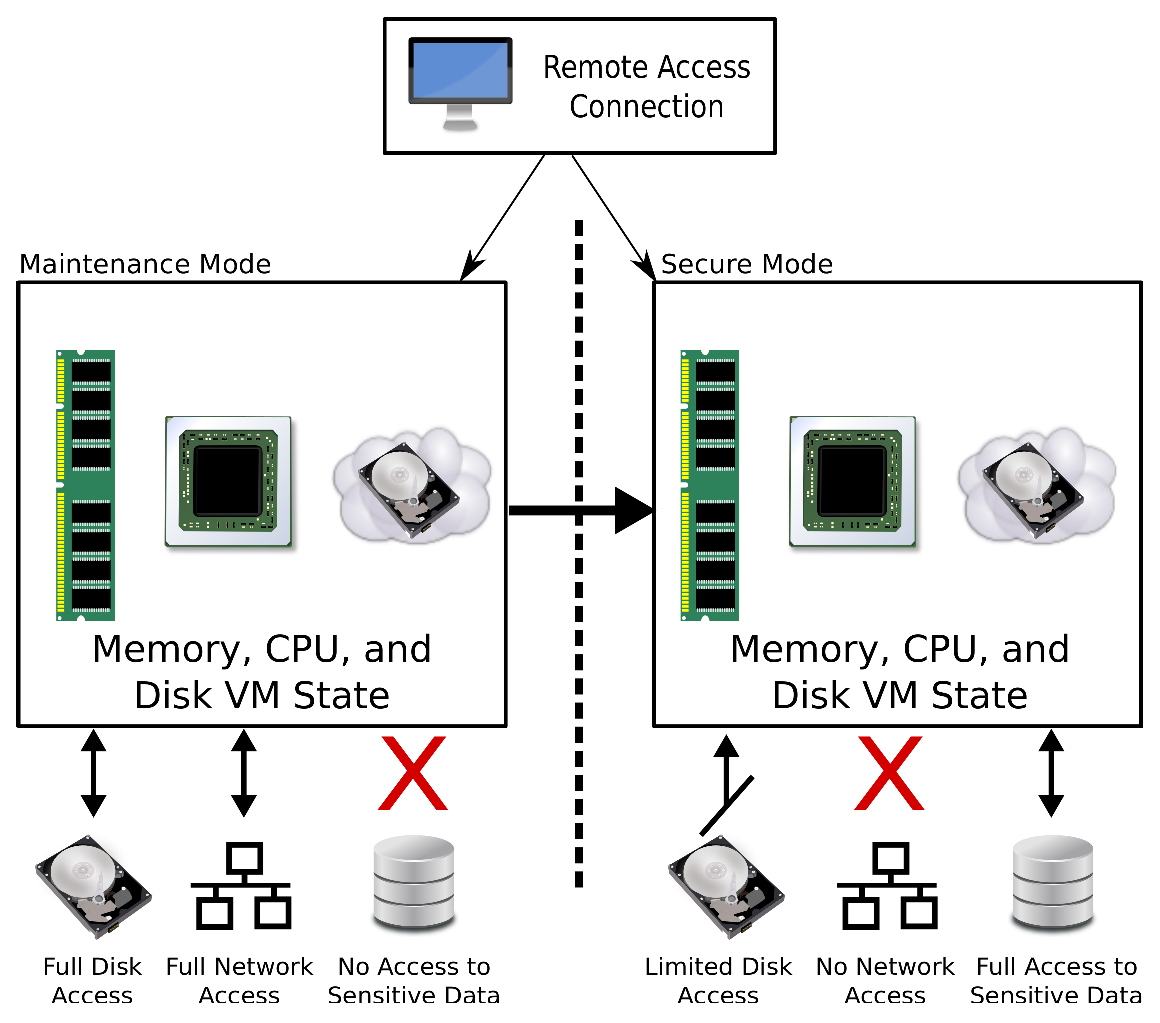
\includegraphics[width=3.0in]{figures/architecture}

\caption{A Data Capsules virtual machine runs in one of two modes.  In
maintenance mode, VM state such as memory, CPU and disk state persists across
shutdowns and mode transitions.  In secure mode, this virtual state is lost
once a user returns to maintenance mode. The only exception is any data stored
in the user's secure storage volume, which is attached to the VM only when the
user enters secure mode.}

\label{fig:architecture}
\end{figure}

Data Capsules features an architecture, illustrated in Figure
\ref{fig:architecture}, that makes heavy use of virtualization.  For each
system user, there are one or more corresponding VMs.  Multiple VMs per user
may be useful in situations where there is a large repository of data that is
separated into multiple corpora each with their own access permissions.  In
this case, a user could potentially have multiple VMs, each with access to a
different corpus.  However, the handling of such an access permissions system
is outside the scope of this paper.

The major element that is used to isolate VMs that are in the middle of
accessing sensitive data is live migration \cite{migration-clark}.  When a VM
switches from maintenance mode to secure mode, the underlying virtual machine
manager migrates that VM to a separate physical machine that has access to the
sensitive data, but which is configured to lack network access for any purpose
other than to receive other incoming VM migrations.  In other words, VMs in
maintenance mode are strictly segregated within separate physical machines from
VMs running in secure mode.  We can therefore refer to a physical machine
running only maintenance VMs as a \emph{maintenance machine}, and likewise a
\emph{secure machine} runs only secure mode instantiations of VMs.  We illustrate an example deployment in Figure \ref{fig:configuration}.

\begin{figure}[ht!]
\center
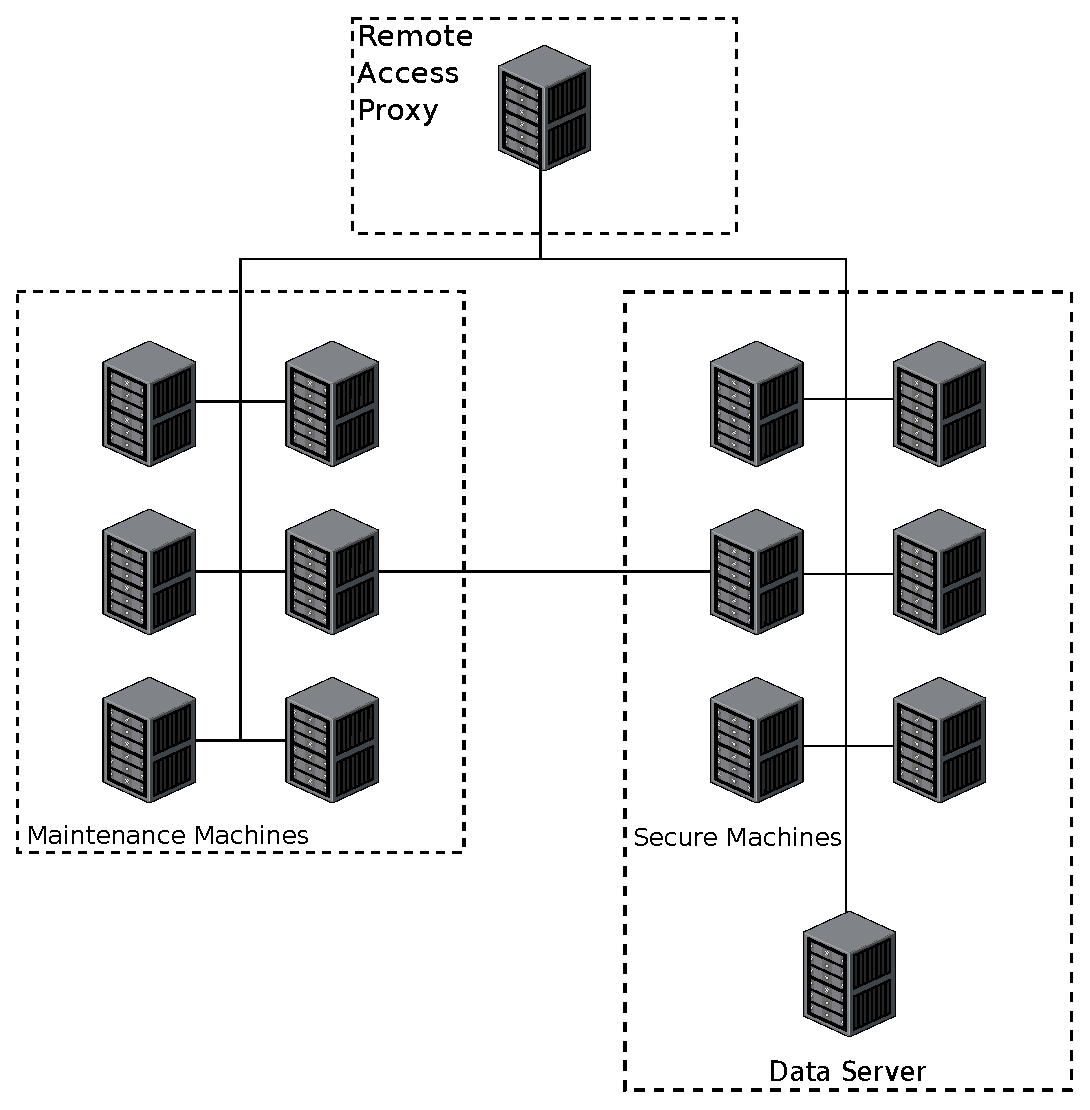
\includegraphics[width=3.0in]{figures/configuration}

\caption{An example deployment configuration for a Data Capsules system.
Dotted boxes denote physical separation, which is necessary between maintenance
machines, secure machines, and the remote access proxy.  The sensitive data
server may exist separately, or it may reside on one of the secure machines.
The only connections between maintenance and secure machines will be for the
purpose of tranferring virtual machine state to secure machines, and for
read-only accesses to the VM disk images.  This data largely travels in one
direction, from maintenance machines to secure machines.}

\label{fig:configuration}
\end{figure}

By adopting this segregated design, the threat of data leak via covert channels
within a single physical machine is eliminated, so long as the trusted computing
base remains uncompromised.  The remaining risk is that of one VM in secure mode
leaking data to another VM that is also in secure mode, but there is no reason
to want to do so, as both VMs would already have access to the entire secure
repository.  On a machine running VMs in maintenance mode, there is no way to
access the sensitive data, and hence no data to be leaked.  We stress that this
design also requires at least two physical machines in order to provide these
security guarantees.

\subsection{Maintenance Mode}

As the name suggests, maintenance mode is intended to allow a user to maintain
their VM's software environment, performing actions such as updating software
and uploading any files needed to conduct their research when in secure mode.
In accordance with these needs, maintenance mode allows the user full Internet
access and persistent storage (i.e.  changes to the virtual hard disk will
persist on reboot) in exchange for a lack of access to the sensitive data and
the user's persistent secure storage volume.

When a user initiates the switch to secure mode, their system state is migrated
to a secure machine.  Once this migration has completed, the state of the
maintenance VM is frozen, and remains in this frozen state until the user exits
secure mode.  Upon exit from secure mode, the maintenance VM is simply unfrozen,
and continues processing from the point at which it left off at the time of the
original switch to secure mode.

\subsection{Secure Mode}

When the user switches to secure mode, the state of their VM, previously in
maintenance mode, is migrated to a secure machine where it continues execution.
By switching to secure mode, the user sacrifices network access and virtual hard
disk storage persistence in exchange for access to the sensitive data and their
secure storage volume, which is mounted upon entering secure mode.  Any changes
to the normal storage are stored only in the machine's virtual memory, and
discarded when the user exits secure mode.  Only changes to the user's secure
storage volume will persist to the next time the user enters secure mode.
Indeed, when the user switches back to maintenance mode from secure mode, all
accumulated state change after the original switch into secure mode is discarded
from memory, and the maintenance VM simply resumes execution from where it left
off prior to the switch.

Conceptually, we can also think of this functionality in this way: by using the
same single virtual machine and transporting it, via migration, to a different
environment where it is subject to a different set of permissions and
privileges, we can allow the user to transport a custom software environment
created in an insecure environment over to a secure environment where it can
then be used to conduct research, and subsequently be discarded.  By giving them
a secure storage volume in secure mode, the user can save their intermediate
results before further iterating their software environment, preserving
flexibility in the case that they require further enhancements to their
software environment.

The use of two separate modes for a single virtual machine, as opposed to, say,
using two separate machines or two separate VMs, allows the user to customize
the software environment they use when the secure data is accessed.  This would
not be possible without opening high-risk channels or a burdensome and
inconvenient auditing process under a two (virtual) machine model.

\section{Implementation}
\label{sec:Implementation}

A prototype of the Data Capsules system has been developed using the KVM virtual
machine manager, which is built in to the Linux operating system, along with the
user-level counterpart application qemu to achieve virtualization.  A set of
Bash shell scripts were written to implement the basic operations for managing
Data Capsules VMs.  Although the current prototype does not fully support the
migration-based mode change described in this paper, migration-based switching
has been implemented and demonstrated, and the only remaining work is to fully
integrate it into the existing code.

End users may use either a convenient web interface, or call the scripts
directly in order to perform basic operations including creation and deletion of
VMs, running and stopping VMs, as well as switches between maintenance and
secure modes.

Although it could be argued that other, better choices for a virtual machine
manager exist on which to base such a demonstration system, it is the opinion of
the authors that no currently existing virtual machine manager is sufficiently
well written and designed so as to serve as an ideal choice, since there is no
x86-based hypervisor that is formally proven to be properly implemented and
secure.  The choice of KVM was for its ubiquity as part of the Linux operating
system along with ease of development.  However, as mentioned in Section
\ref{sec:Threat Model}, microkernels do exist which serve to demonstrate that
at least something close to such a robust, well-designed VMM could be made.

\subsection{Network Protections}

The Data Capsules prototype uses iptables rules to implement a simple set of
firewall rules for VMs.  All VMs on a machine reside on a bridged, private
network.  In secure mode, additional rules are imposed on the private IP address
of the VM, restricting all network access except that between the VM and the IP
address of the one or more servers containing the sensitive data, as written in
a simple configuration file.  

Because limiting access to only a small set of servers eliminates access to
public DNS servers, for our prototype we configured the \texttt{/etc/hosts}
file on VM images to allow them to resolve the server domain names when in
secure mode.  More elegant solutions could be achieved by allowing access to a
custom purpose-built DNS server, or by using solutions like
cloud-init\cite{cloudinit}, which is available for Ubuntu-based virtual
machines.

\subsection{Secure Storage Volume}

In order for a user's intermediate research to persist across sessions within
secure mode, a storage volume is attached upon entering secure mode.  This
volume is implemented as a disk image file, which is attached as an emulated USB
thumb drive.  From the user's perspective, this is a convenient access paradigm,
as one can imagine a virtual USB drive being ``plugged in" to the machine when
the user switches to secure mode, and then being removed when the user switches
back.

One currently unresolved issue with this approach, and any using a mounted disk
volume, is the issue of caching by the operating system of any changes to the
secure volume.  Since changes typically are not immediately written back to a
disk volume, this raises the possibility that a user could switch out of secure
mode before all data is written back, resulting in data loss.  Currently, we
warn users of the prototype before they switch out of secure mode that they must
detatch the secure volume or risk data loss.  In the future, we might include
software on preconfigured VMs that can help users know when it is safe to switch
out of secure mode.

\subsection{Releasing Research Results}

Since users ultimately require some method for releasing the results of their
research, qemu was configured to create a channel through the serial port on the
VM to a UNIX domain socket on the host machine.  A simple daemon was written
which runs on the secure machine to listen on this socket for any results to be
released.  It follows an extremely simple protocol that takes the file name,
file size, and file data and exports them to a database where they can then
undergo a review process.  We discuss a potential approach for automating this
review process for candidate release data in Section \ref{sec:Results Audit}

\section{Discussion and Future Work}
\label{sec:Discussion}

Although a basic prototype has been implemented and is fully functional, there
are still many potential routes for improvement.  We discuss many of these,
including some we are currently investigating and some that we intend to look
into in the future.

\subsection{Securing Client Access}

As mentioned in Section \ref{sec:Threat Model}, the channels used to access a VM
are an important element that must be secured in order to safeguard any private
data.  In the event of more sophisticated attacks, such as a man-in-the-middle
attack between the end user and the Data Capsules infrastructure or a compromise
of the end user's device, it is not hard to conceive of very powerful attacks.

For instance, if an end user's device is compromised, the malicious party could
then install malicious software on the VM while in maintenance mode that is
designed to enter secure mode and subsequently encode all of the private data in
the format of the channel medium (e.g. as an image in the case of remode desktop
protocols like VNC).  The data could then be decoded by additional software
running on the compromised client, or even forwarded for decoding on the
attacker's personal infrastructure.  In the case of a 1024x768 screen resolution
refreshing at 15 times per second, an attacker could leak over 2 GB of data from
a protected repository within one minute, or at the very least saturate the
channel connection with the leaked data.

This example clearly illustrates the imperative need to secure the remote access
channel from these types of attack.  There is also, however, a limit to what can
be done, since the user ultimately must have some way of seeing into the VM that
they are remotely administering.  The first obvious step is to secure the
client-server connection using SSL with certificate-based authentication.  While
this would seem trivial to accomplish, there is an unfortunate lack of support
for such a secure connection in existing widely used VNC clients.  We are
currently in the process of modifying an existing VNC client to support SSL
connections with certificates.  Beyond this initial setback, we expect
implementation to be relatively trivial.

Beyond securing the connection, we are currently investigating methods for
securing the end client device using the Trusted Platform Module (TPM)
\cite{tpm} on an end user's device to remotely attest that the end client is
secure.  We envision the final implementation will consist of a USB thumb drive
containing a barebones Linux operating system with an installed VNC client, and
will use the TPM's features to perform a measured boot of Linux and the VNC
client.  Users will plug in the USB drive to their device and boot into the
secure environment in order to access their Data Capsules VMs.  In this way, we
hope to greatly raise the bar for a malicious attacker who wishes to gain
access to sensitive data, while preserving a reasonably uncumbersome method for
access to the end user.

\subsection{Partial Automation of Release Auditing}
\label{sec:Results Audit}

Although Data Capsules aims to ease secure access to sensitive data by removing
the need to audit data and software being imported into a secure environment, it
does not address how to ease the auditing of results data being released from
that same environment.  This is a challenging issue, since a careful attacker
could use any number of methods to disguise the leaking of large amounts of data
as something that appears entirely innocent.

While there is no evident solution, there are likely many measures that could be
taken to automate the identification of more obvious leak attempts.  For
example, simply measuring the information content of a candidate for release,
say by measuring its Shannon entropy or its compressed file size, if the
candidate is unusually large then it may be immediately flagged as suspicious.
This is only the tip of the iceberg, and there are likely more elegant and
powerful solutions available.  We leave investigation into such a system as
future work.

\subsection{Optimizing Mode Switches}

As mentioned in Section \ref{sec:Implementation}, the migration-based mode
switch has currently been implemented as a demonstration, and has yet to be
fully integrated into the prototype.  We are currently addressing two
issues that will help usability and performance of this key element.

The first of these issues is the fact that migrating a VM across two physical
machines currently requires the user to reestablish a remote desktop or shell
connection with the destination machine.  We intend to set up a proxy connection
system that will redirect the user's connection automatically, without the need
for any action on the user end.  Such a proxy would need to reside on a machine
separate from machines serving VMs, otherwise it would create an intermachine
covert channel, since there would at some point be a connection link between a
process on a maintenance machine and a process on a secure machine.

The second issue with designing a mature migration-based mode switch is that of
speed and performance.  Transferring the state of many machines all running in
maintenance mode could easily strain even a very robust network.  Therefore it
is likely that some form of rate limiting will need to be imposed in order to
relieve network pressure.  The consequence of this is of course that the time it
takes to switch modes will increase.  We therefore plan to investigate to find
the best compromise between the two needs of limiting use of network bandwidth
and maximizing switch performance.

\subsection{Evaluation}

Since the ultimate goal of the Data Capsules system is to improve usability of
remote access to sensitive data, it is natural that performance is an important
measure of its success.  Virtual machines must not suffer any slowdown, and the
new mode switching interface that it introduces must not be inconveniently slow.
Additionally, direct feedback from actual users of our system can serve as a
useful measure of its merits in practice.

\subsubsection{Performance}

Fortunately, virtual machine performance is not significantly affected by Data
Capsules, since it requires no significant changes to qemu or KVM.  Basic VM management functions also run quickly, with starting and stopping and deleting VMs taking only fractions of a second.  VM creation has also been made almost instantatneous to the user through clever use of copy-on-write references to base disk images.  This leaves only the performance of switches between modes.

For our evaluation, we plan to consider two useful measurements for assessing
the speed of a migration-based mode switch.  Since VM state begins to be
transferred to the target secure machine immediately upon startup, there is a
time from startup until the state transfer tapers to a steady stream as most of
the initial state is completely transferred and only new updates are then
carried over.  In our tests on two servers linked by a direct wired connection,
this switch \emph{startup time} took about 20 seconds for a base installation of
Ubuntu 10.04, which took about 3.5 GB of virtual disk space.  We note that the
entire virtual hard disk contents are not transferred, but only copy-on-write
changes to the virtual hard disk, as well as the entire contents of memory and
CPU registers.  This startup time is easily approximated by the actual execution
time of a normal, undelayed migration between two machines.

The second element is the actual \emph{execution time} of a switch, assuming
that the aforementioned startup process has already occurred and there is only a
small amount of update data that is being periodically generated and
transferred.  So long as the end user has used a machine for a time greater than
the startup time, and so long as bandwidth is not constrained so much that the
new data being generated cannot fully transfer within the window in which it is
generated, then there should only be a small, negligible delay, that is
virtually imperceptible to the user.

For our existing prototype, which does not use migration-based mode switches,
but rather makes use of VM live snapshots, it is not inaccurate to say that its
functionality is comparable to that of a migration-based mode switch without the
delay of transferring state across machines.  In this sense, the execution time
of a snapshot-based mode switch should certainly be no less than the execution
time of an equivalent migration-based execution time.  In light of this, we can
use the mode switch performance time for a snapshot-based mode switch to
approximate the upper bound for switch execution time in the final
migration-based Data Capsules system.  In practice, we have observed that this
switch time almost always falls within 5 seconds, and is usually closer to 1 or
2 seconds.

We also note for clarity that these switch times refer to the switch from
maintenance mode into secure mode.  Under a migration-based mode switch, the
switch back to maintenance mode simply requires unpausing a VM and switching
back the remote desktop or shell connection to the maintenance machine that VM
is running on.

\subsubsection{User Study}

A user study is another important option for evaluating the undeniably
unfamiliar paradigm of having two machine modes for a single conceptual machine.
Although we have no plans to conduct a formal study in the near future, we are
in the process of implementing a prototype of the system that will be used by
humanities researchers for secure access to copyrighted materials.  After
initial alpha testing by a small number of subjects unfamiliar with the system,
feedback was positive, with no apparent complaints or confusion about how it was
used.  We leave more formal and in depth user studies for future work.

\section{Conclusions}

In this paper, we introduced Data Capsules, a system that enables more usable
access to sensitive data repositories by eliminating the need to audit data and
software that are brought in to the secure environment.  Data Capsules presents
users with a maintenance mode for fully customizing their software environment,
and allows users to then import this environment into a secured environment
where they can then perform analysis on sensitive data with limited risk of data
leak.  Data Capsules achieves this mode paradigm by migrating underlying VMs
between machines segregated by their access to the network and to the sensitive
data.  A prototype of the system has been implemented, and initial performance
data and end user feedback are both promising.

% References
\bibliographystyle{abbrv}
\bibliography{paper}

\end{document}
